%add a portion of graph to explain
% \begin{enumerate}
%     \item \textbf{}: a control flow graph which represents calling relationships between functions in a program. Each node represents a procedure and each edge (f,g) indicates that procedure f calls g. A circle in the graph indicates recursive procedure calls. Profiler outputs dynamic call graphs that represent this run of the program.
%     % \item \textbf{Flame Graphs}: A visualization tool for stack traces, commonly to visualize cpu profiling. The \textit{x} axis shows the stack trace collection, they are alphabetically sorted from left-to-right and have no relation with time. The \textit{y} axis shows the stack depth, ordered from root at the top to leaf at the bottom. The width indicates the frequency of the trace, wider boxes were more present in stack traces. Each column of boxes is a stack trace and each box represents a stack frame, that is a function.
%     % \cite{flamegraphs}
% \end{enumerate}

% \begin{figure}
%     \centering
%     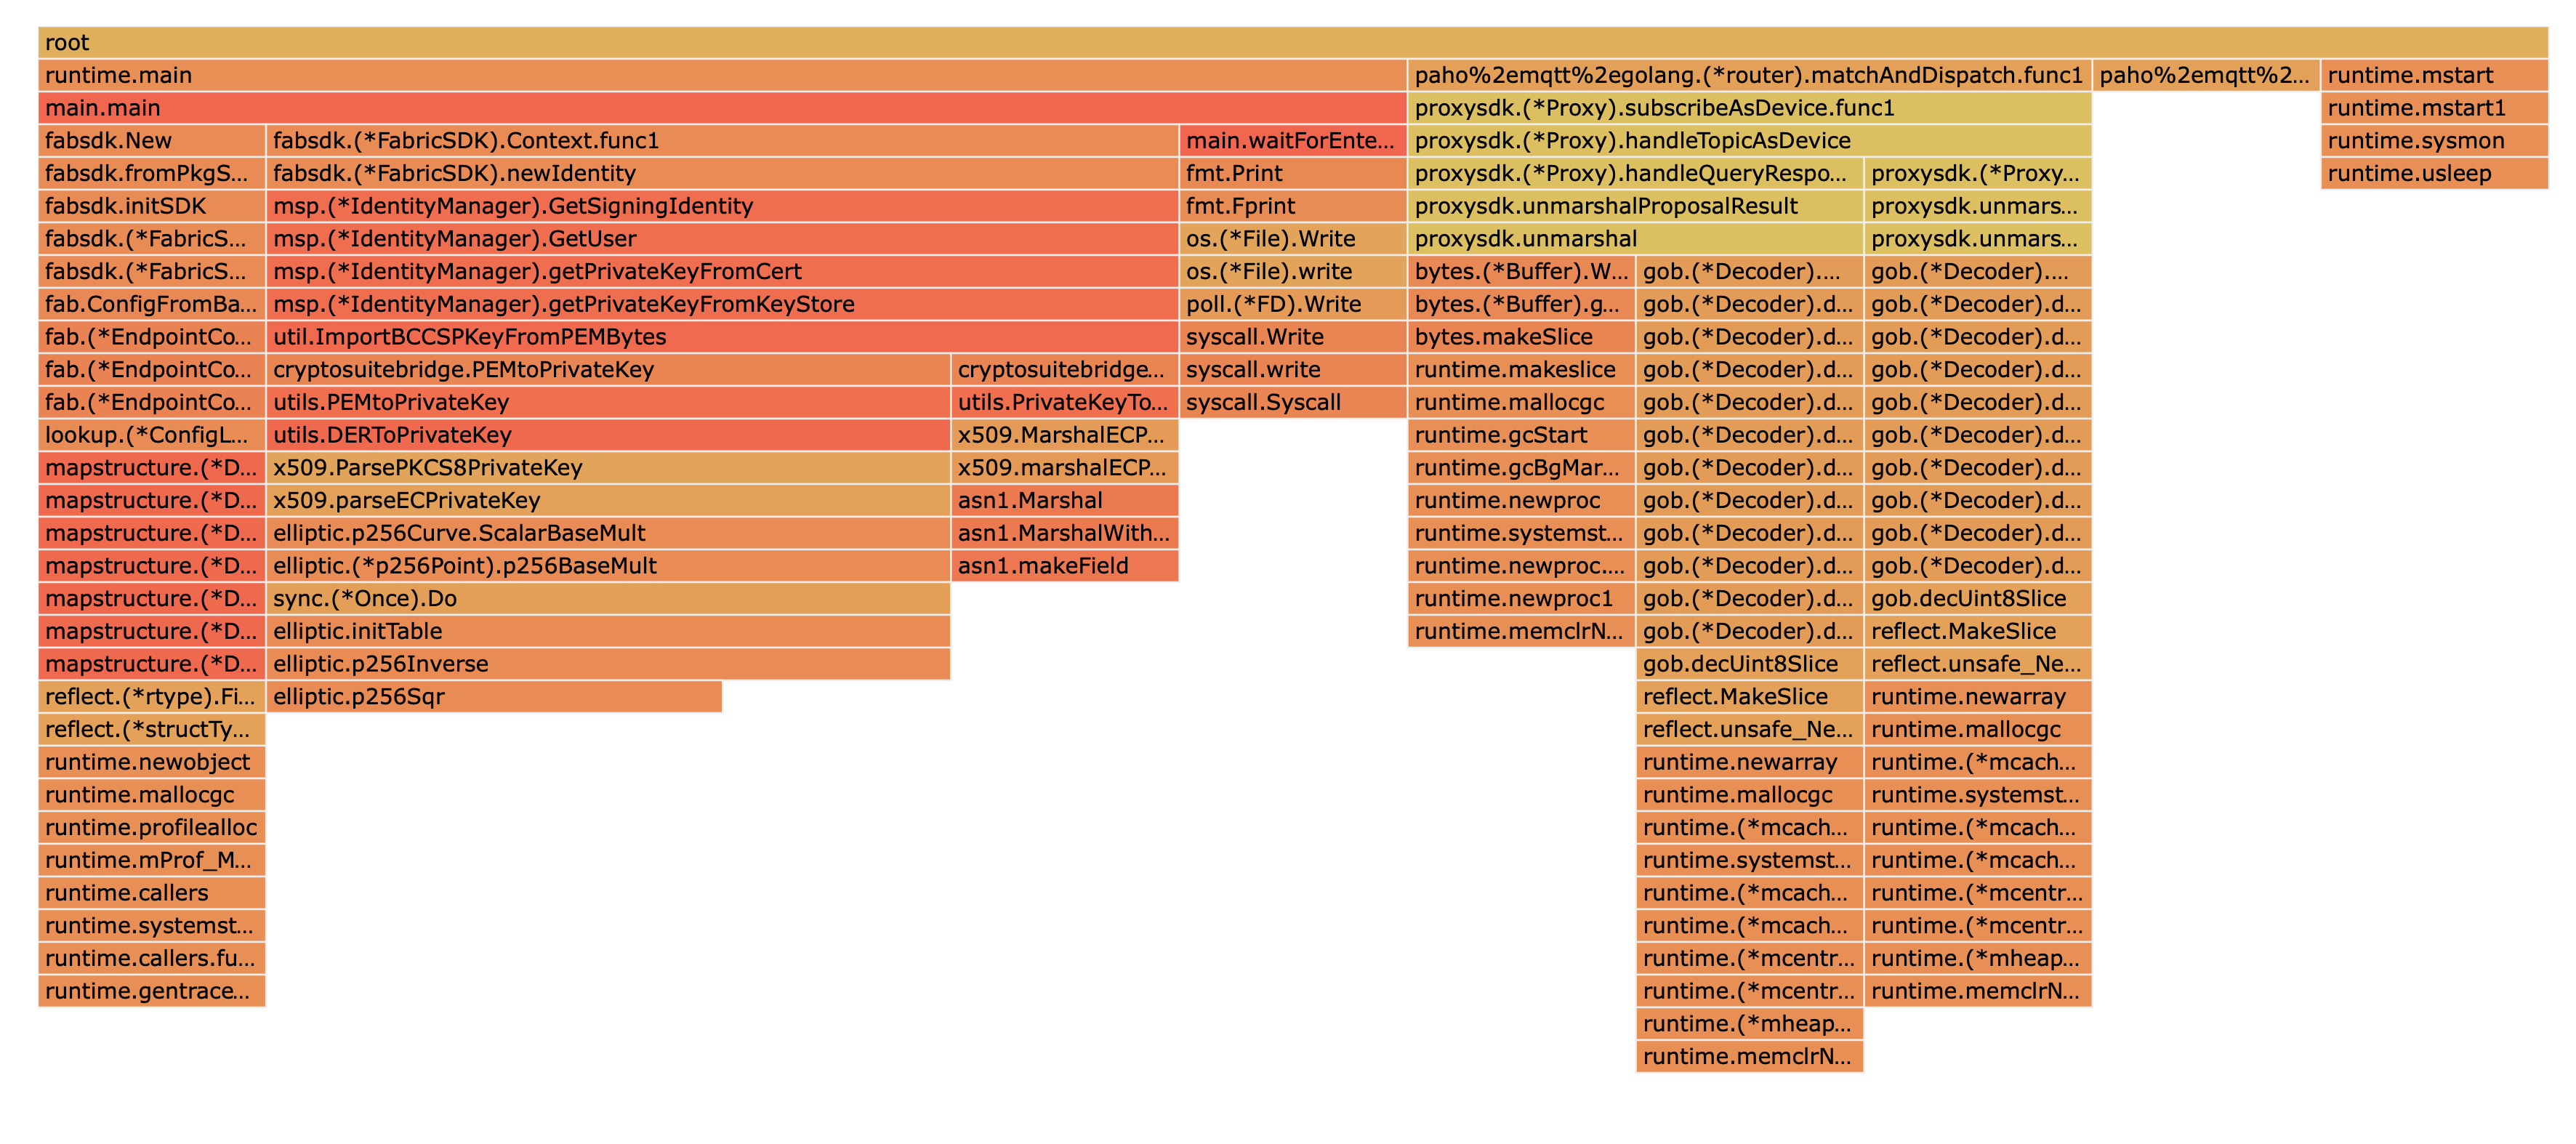
\includegraphics[width=1\textwidth]{images/6_performance/flamegraph-cpu.png}
%     \caption{Flamegraph of client}
%     %What do we observe here? What is the use of this graph? Check other flame graphs
%     \label{fig:cpu-prof-flame}
% \end{figure}